\section{Results}

\mike{Results and Discussion:}
\begin{itemize}
    \item (Overview) Give an overview of results, possibly referencing a graph or two.
    \item Statistical analysis: provide positive and null hypotheses for the research questions.
    \item Evaluation of research questions: statistical results and explanations of the graphs.  One subsection per research question?
    \item Threats to validity: what are our threats?
    Internal validity: not really necessary, I think.
    External validity (how much can the results be generalized):
        1. currently all models are *very small*;
        2. Many programs were drawn from mutations of a relatively small number of ``seed'' programs;
        3. The models are written in Lustre rather than FOL.  This means that the
            top-level conjunctions are all over equations rather than general
            form;
        4. Others?!?
    Construct validity: we are measuring what we think we're measuring: IVC and minimality are reasonably defined.  For discussions of ``completeness'' and ``traceability'' we need to be clear about any claims (probably not in this paper).
\end{itemize}

\mike{In general, I do not think we are asking quite the right questions yet.  More feedback will come tomorrow}


To evaluate the dependency of our algorithm on different solvers and engines, for each LUS model, \texttt{JKind} was run with 13 different configurations and a timeout of 700 seconds. We chose four SMT solvers: \texttt{Z3}, \texttt{Yices}, \texttt{MathSAT}, and \texttt{SMTInterpol} as well as three engine configurations: \texttt{PDR},
\texttt{K-induction}, and both of them. In other words, the \texttt{ReduceSupport} engine was run with 12 combinations of those settings. And, one additional configuration is where \texttt{JSupport} computes a minimal support set. Therefore, experiments are based on these $405 \times 13 = 5265$ \texttt{JKind} runs. It is worth mentioning that we were to add randomness to the solvers and extend these 13 configurations. However, after performing some initial experiments and analyses, it turns out that random-seed in solvers does not affect the output of our algorithm; hence, it was not considered in the configurations.\footnote{The benchmarks and all the raw experimental results are available on \cite{expr}. The directory also contains mined data obtained from the raw results.}

%\ela{we may want to remove this part}

With a 700 second timeout, 10 models had unknown property. In other models with valid properties, for 112 models, all solvers with \texttt{K-induction} setting failed to prove the properties. That is to say, in $(112 \times 4) + (10 \times 13) = 578$ runs, \texttt{JKind} was unable to to prove the property, so the set of support in those runs remained unknown as well. As far as \texttt{JSupport} concerned, support computation in 18 models timed out (with 700 second limitation).

\subsection{Evaluation}
\label{subsec:eval}
\section{Evaluation}
\label{sec:eval}
This section evaluates our approach by addressing the following research questions:

\ela{could you please rephrase these questions?! having hard time saying them clearly :-( }
\begin{itemize}
    \item \textbf{RQ1:} How much overhead does computation of set of support add to the proofs? 
    \item \textbf{RQ2:} How dependent is our approach on different tools and proof engines? Does different solvers/ proof engines generate different support set? If so, to what extent are they different?
    \item \textbf{RQ3:} Is there any relationship between the size of a computed support set and 
    solvers/ proof engines? 
    \item \textbf{RQ4:} Is there any relationship between the size of the model and the variety of support sets?
    \item \textbf{RQ5:} How close to minimal are the support sets computed by our algorithm? For each model, we have 12 sets of support computed by \texttt{JKind}, and one \emph{minimal} set computed by \texttt{JSupport}; we would like to know which configurations generated sets that are very close or far to the minimal one.
    \item \textbf{RQ6:} How do different solvers perform on computing support? And, how efficient is it in comparison with \texttt{JSupport}?
\end{itemize} 

\subsection{Analytical Results}
\label{sec:res}
This section answers the aforementioned research questions briefly describing the way the results are analyzed. Note that the results of 10 models with unprovable properties are omitted in calculations. In addition, while analyzing support sets, \texttt{K-induction} settings that timed out were not considered because they failed to prove the properties. 

In general, for timing analyses, from all 13 configurations, we only considered the settings where both \texttt{PDR} and \texttt{K-induction} engines were activated. Since this configuration is a default setting in \texttt{JKind}, we only care about timing while both engines are employed. Therefore, $(4 \times 405) = 1620$ of all 5265 runs have been analyzed to address time-efficiency questions.


% RQ1: the overhead of support computation on different solvers
\textbf{RQ1.} The overhead is defined as the percentage of the overall runtime is dedicated to support computation:

\mbox{$overhead\_percentage = 100 \times (support\_runtime \div overall\_runtime)$}

 Table~\ref{tab:overhead} shows the overhead of support computation on different solvers.


\begin{table}
  \centering
  \begin{tabular}{ |c||c|c|c|c| }
    \hline
     solver & min & max & mean & stdev \\[0.5ex]
    \hline
    Z3   & 0.726\% & 45.396\% & 13.414\% & 11.369\% \\[0.5ex]
    Yices &   0.200\%  & 262.254\%   & 47.264\% & 51.193\% \\[0.5ex]
    SMTInterpol& 0.930\% & 268.571\% &  70.500\% & 58.541\%\\[0.5ex]
    MathSAT & 0.502\% & 396.124\% &  71.007\% & 79.990\%\\[0.5ex]
    \hline
  \end{tabular}
  \caption{\small{Overhead of support computation on different solvers}}
  \label{tab:overhead}
\end{table}

\vspace{6pt}
\noindent\fbox{%
    \parbox{\textwidth}{%
        In average, computation of support set has less than 50\% overhead. Averagely, if it takes \textit{t} to prove $\mathbb{P}$, it will take \textit{1.5t} to both prove $\mathbb{P}$ and compute its set of support.
    }%
}
 \vspace{9pt}

% RQ2: How dependent is our approach on different tools and proof engines?
\textbf{RQ2.} To answer this question, we analyzed the results from different aspects. The following describes methods used for analyzing and their results.

\textbf{(1)} For each model in the benchmark, the experiments generated 13 different sets of support. We used Jaccard distance to measure dissimilarity between pairwise of these sets:

\begin{center}
$d_J(\small{A}, \small{B}) = 1 - \frac{|A \cap B|}{|A \cup B|} ,\hspace{9pt} 0 \leq d_J(\small{A}, \small{B}) \leq 1$
\end{center}
\vspace{6pt} 

Therefore, we obtained $\binom{13}{2} = 78$ combinations of distances per model. Then, minimum, maximum, average, and standard deviation of the distances were calculated (Fig~\ref{fig:jacdis}), by which, again, we calculate these four measures among all 405 models. The following summarizes the result of this analysis:
\begin{itemize}
  \item Minimum Jaccard distance among all models is: 0.0 
  \item Maximum Jaccard distance among all models is: 0.882 
  \item Average Jaccard distance among all models is: 0.027 
  \item Standard deviation of Jaccard distance among all models is: 0.062 
\end{itemize}


\begin{figure}
  \centering
  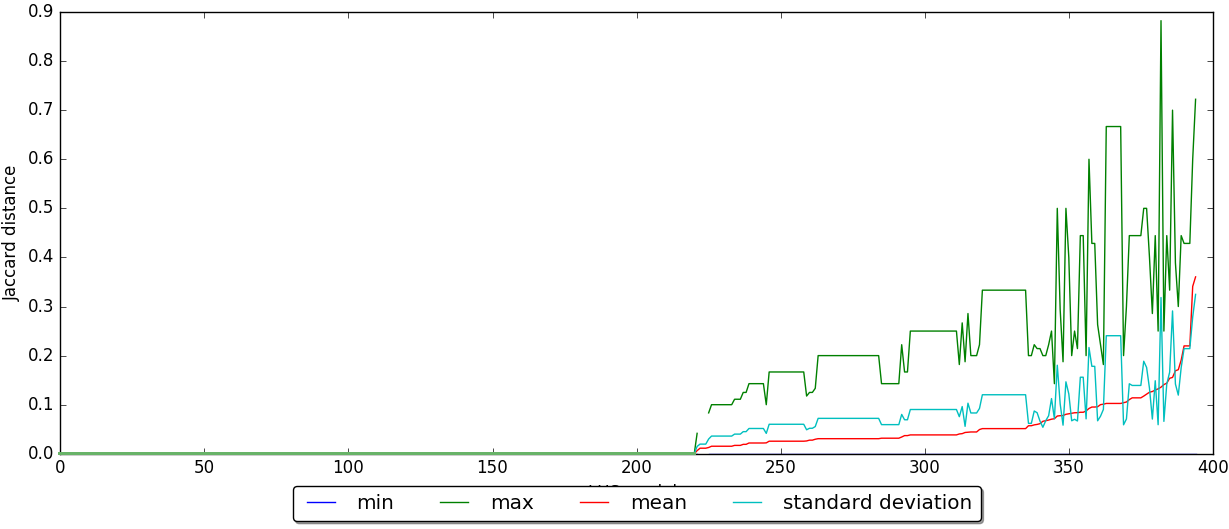
\includegraphics[width=\textwidth]{figs/jacdis.png}
  \caption{\small{Pairwise Jaccard distance between support sets}}\label{fig:jacdis}
\end{figure}

\vspace{6pt}
\noindent\fbox{%
    \parbox{\textwidth}{%
        Support sets computed with different solvers and engines have an average Jaccard distance of 0.027, which implies our algorithm has very small dependency on tools and proof algorithms.
    }%
}
 \vspace{9pt}
 
\textbf{(2)} Since one goal was to know to what extent computed support sets are different, and which configurations have generated more different/similar sets. We analyzed the results,
and it turns out 174 models of 405 contain at least two different support sets (which means in 231 models, all 13 sets of support are the same). We analyzed those 174 models; for each of them, pairwise Jaccard distance between sets was compared, and configurations with maximum/ minimum distances were collected. Fig~\ref{fig:maxdis} and Fig~\ref{fig:mindis} show the results. For example, in Fig~\ref{fig:maxdis}, in 20 models out of 405, \texttt{JSupport} and the configuration where \texttt{Z3} and both proof engines were employed, Jaccard distance between support sets computed by them is maximum. As you can see, different configurations of \texttt{JKind} do not affect very much the variety of the generated sets. However, \texttt{JSupport} and \texttt{JKind} configurations have had maximum distances most of the time. Even so, the frequency of such maximum distances among 405 models is very low.


\begin{figure}
  \centering
  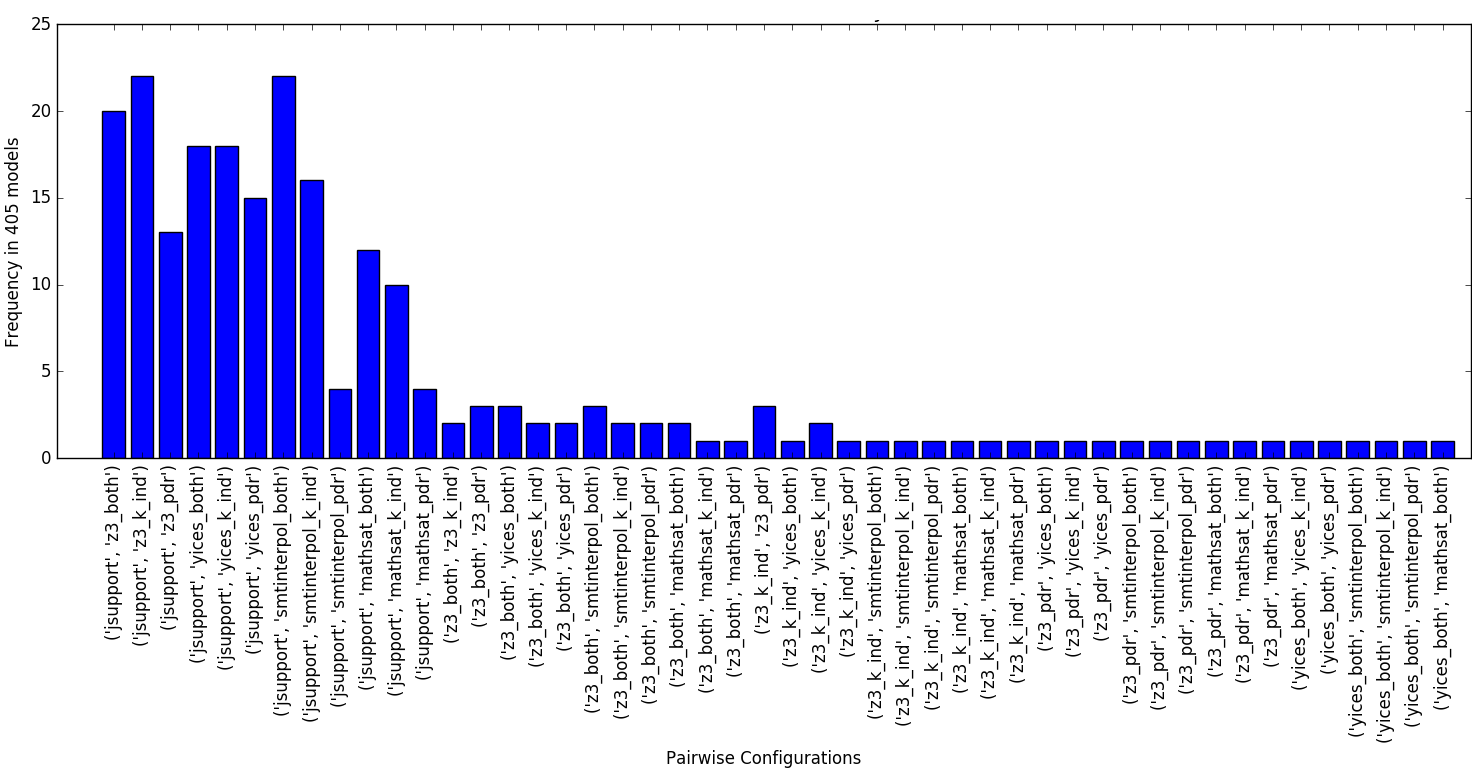
\includegraphics[width=\textwidth]{figs/max_settings_analyses.png}
  \caption{\small{Pairwise configurations with maximum Jaccard distance}}\label{fig:maxdis}
\end{figure}


\begin{figure}
  \centering
  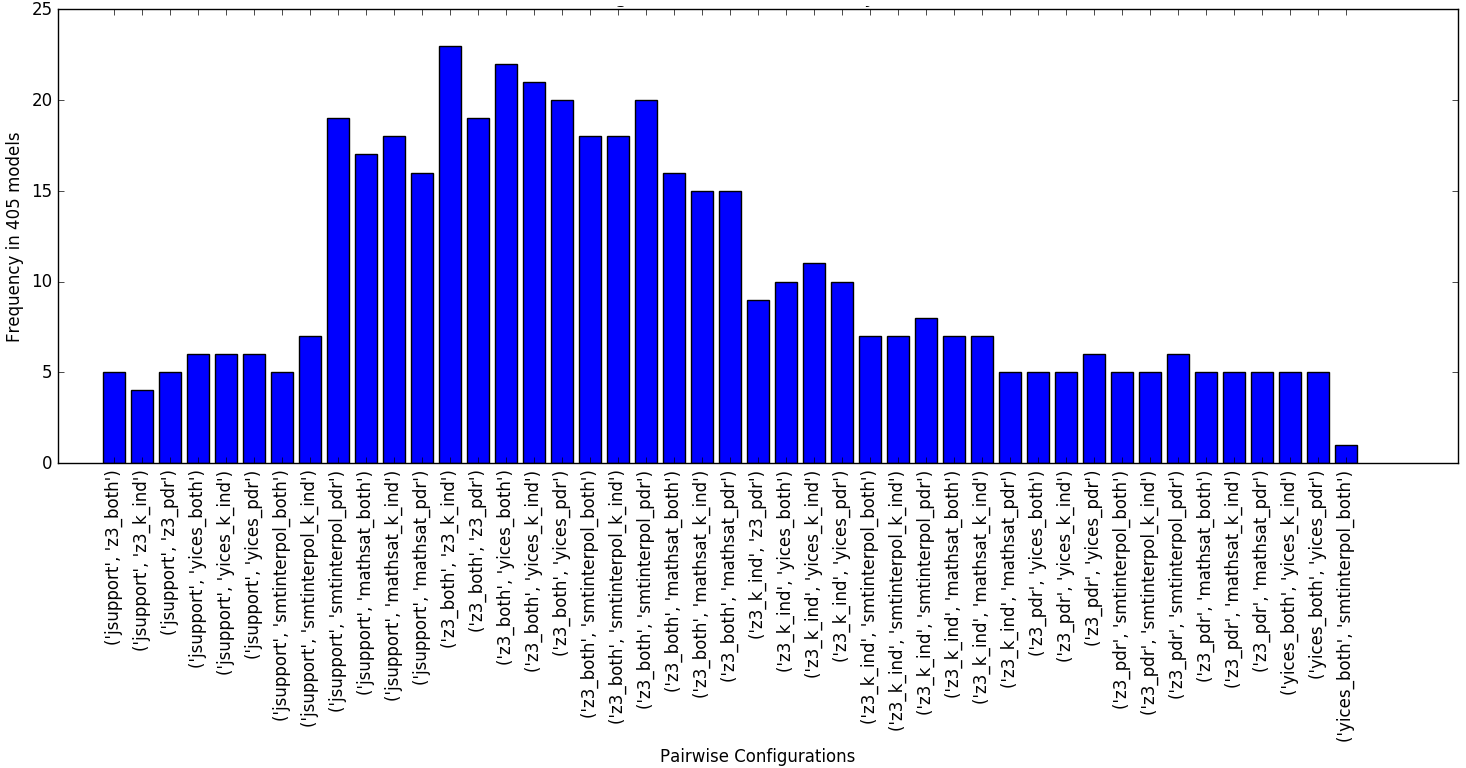
\includegraphics[width=\textwidth]{figs/min_settings_analyses.png}
  \caption{\small{Pairwise configurations with minimum Jaccard distance}}\label{fig:mindis}
\end{figure}

\vspace{6pt}
\noindent\fbox{%
    \parbox{\textwidth}{%
        Different solvers and proof engines have very small impact on the variety of elements in a support set of a property computed by our algorithm.
    }%
}
 \vspace{9pt}

\textbf{(3)} In addition to Jaccard distance, we also measured the similarity among all sets computed in different configurations per model. Let $S_M$ be a set of all support sets computed for model $M$ (i.e. in our experiments, $S_M$ is a set of 13 sets).  We define similarity per model as follows:

\begin{center}
$similarity = \frac{|\bigcap_{i=1}^{13} s_{Mi}|}{|\bigcup_{i=1}^{13} s_{Mi}|}, \hspace{9pt} s_{Mi} \in S_M$
\end{center}
\vspace{6pt} \ela{should see if this formula has any name in mathematics?!}

Needless to say, $0 \leq similarity \leq 1$, and if all the sets in $S_M$ are the same, \textit{similarity} will be 1. So the closer to 1 it is, the more similar sets we have. Fig~\ref{fig:sim} shows similarity in all models. Here is also a summary of minimum, maximum, average, and standard deviation of similarity among all models:
\begin{itemize}
  \item minimum similarity among all models is: 0.12
  \item maximum similarity among all models is: 1.0
  \item average similarity among all models is: 0.884
  \item standard deviation of similarity among all models is: 0.165
\end{itemize}


\begin{figure}
  \centering
  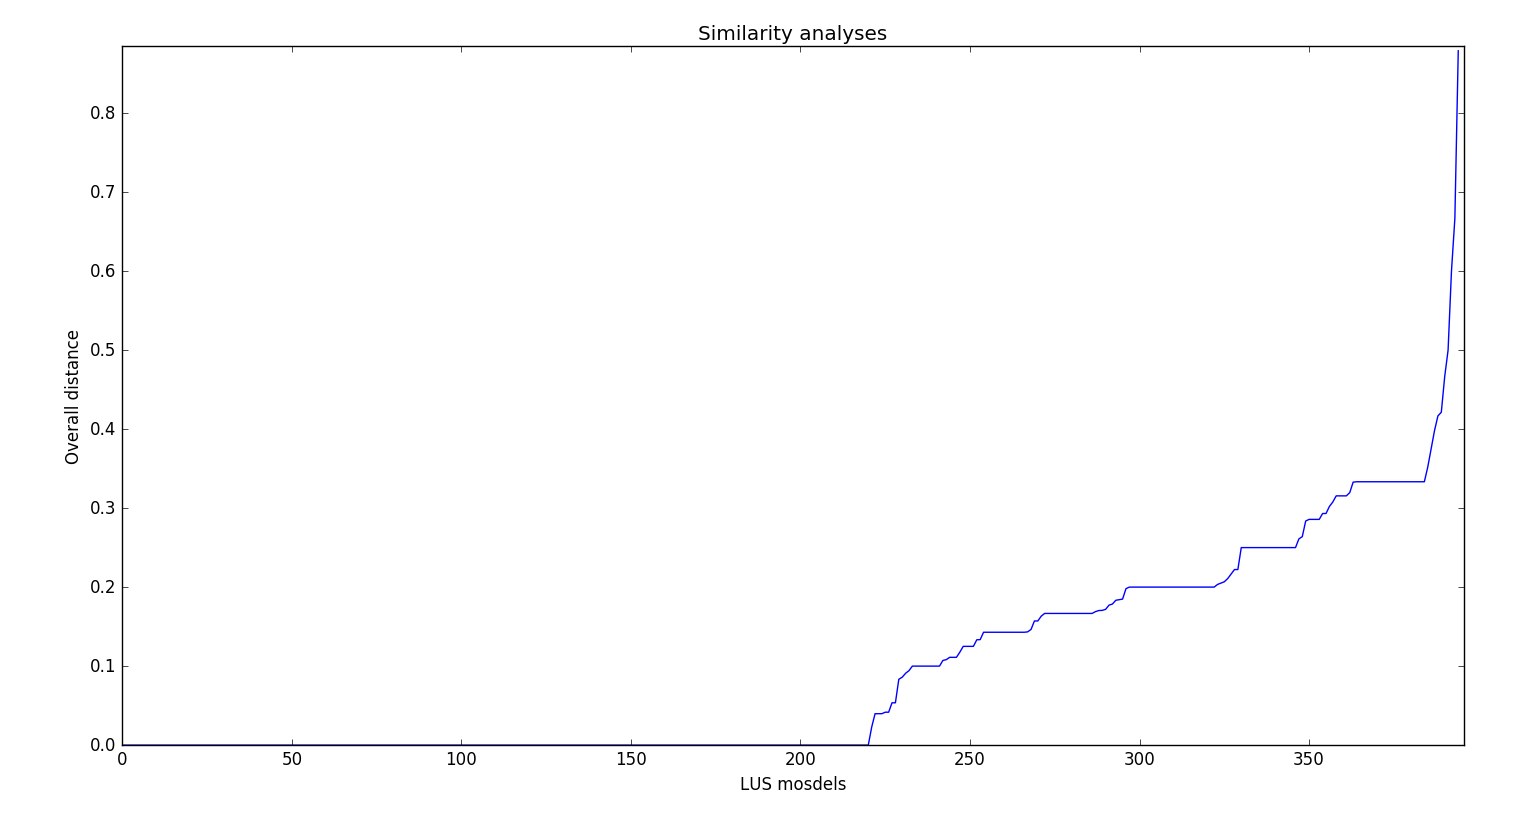
\includegraphics[width=\textwidth]{figs/similarity.png}
  \caption{\small{Similarity measurement for all models}}\label{fig:sim}
\end{figure}

\vspace{6pt}
\noindent\fbox{%
    \parbox{\textwidth}{%
        An average \textit{similarity} of 0.884 shows that support sets computed in different 
        configurations are very similar. So, the dependency of our algorithm to different solvers and proof engines is negligible.
    }%
}
 \vspace{9pt}

\textbf{(4)} We also calculated a \emph{core} support set for each model of the benchmark; A core set of model $M$ is defined as
$\bigcap_{i=1}^{13} s_{Mi},   \hspace{9pt} s_{Mi} \in S_M$. Then, the size difference of the core set with the smallest support set of $M$ was calculated. The results are visualized in Fig~\ref{fig:core}


\begin{figure}
  \centering
  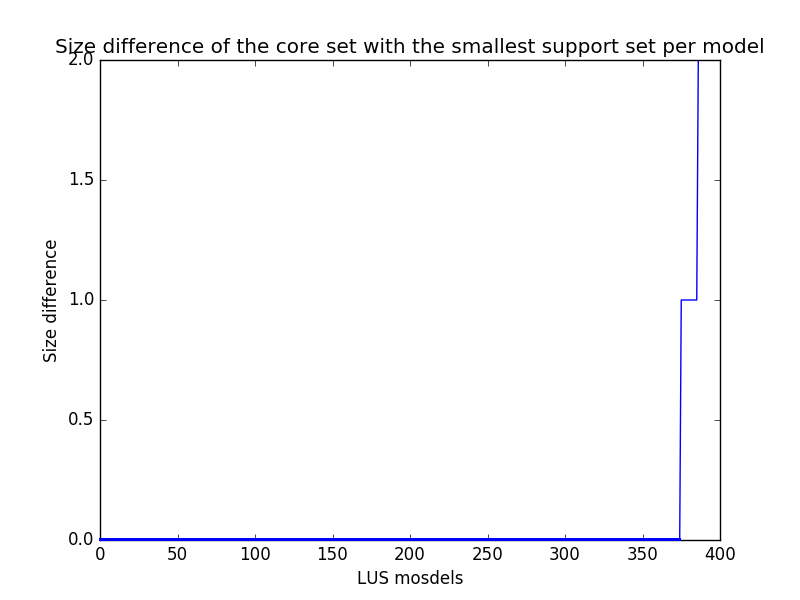
\includegraphics[width=\textwidth]{figs/core.png}
  \caption{\small{Size difference between the core set and the smallest support set per model}}\label{fig:core}
\end{figure}

\vspace{6pt}
\noindent\fbox{%
    \parbox{\textwidth}{%
        The core support set is very close to the smallest support set of a property.
    }%
}
 \vspace{9pt}

% RQ3: Is there any relationship between the size of a computed support set and
%solvers/ proof engines? 
\textbf{RQ3:} To address this question, we analyzed the raw data with two different approaches described in the following.
 
\textbf{(1)} We analyzed the sets of each 405 models. In each model, we looked for configurations that generated the biggest support set and ones that generated the smallest. Fig~\ref{fig:smallest} and Fig~\ref{fig:bigest} visualize the result of this analysis. For example, as you can see in Fig~\ref{fig:bigest}, \texttt{JSupport} generated biggest support sets in less than 10 models. Note that it implies there is at least one \texttt{JKind} configuration that generated the set with a smaller size.


\begin{figure}
  \centering
  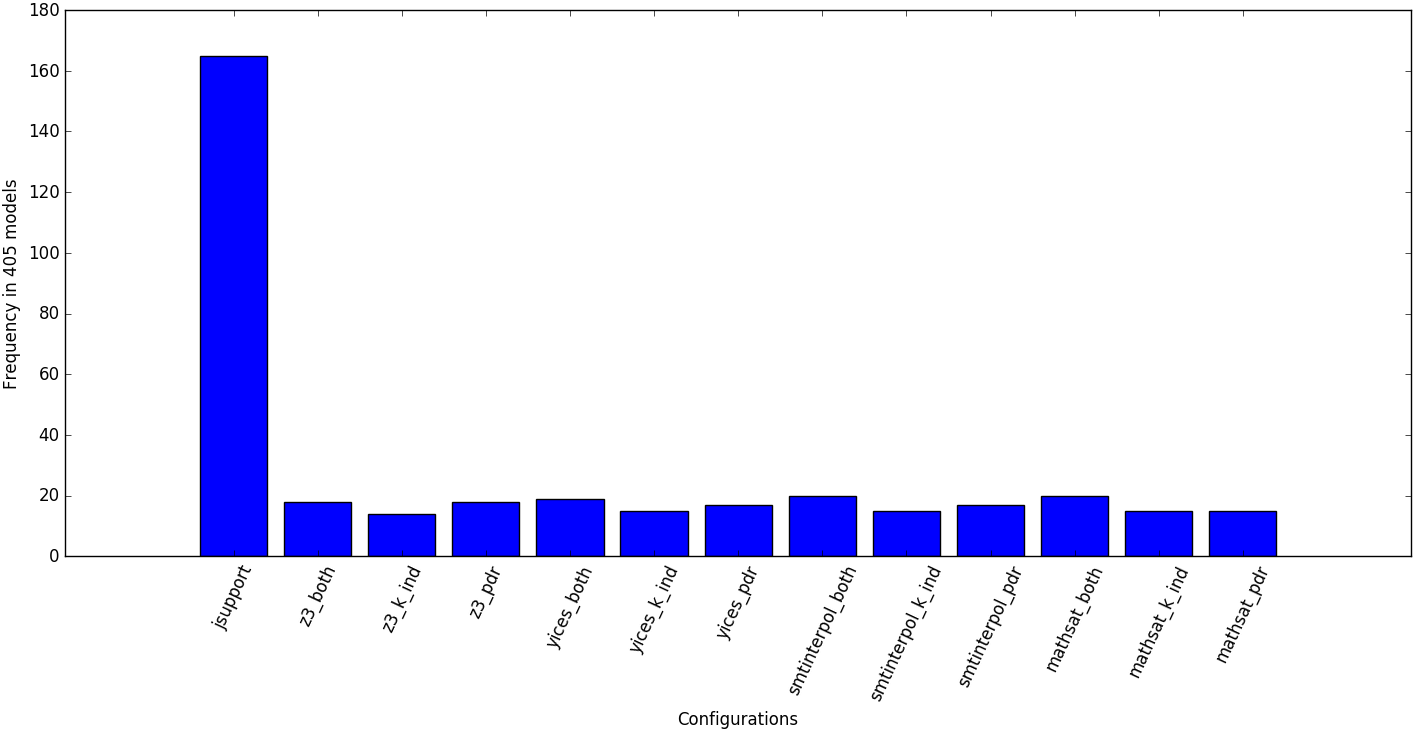
\includegraphics[width=\textwidth]{figs/small_conf.png}
  \caption{\small{Smallest support set (in terms of size) vs configurations}}\label{fig:smallest}
\end{figure}


\begin{figure}
  \centering
  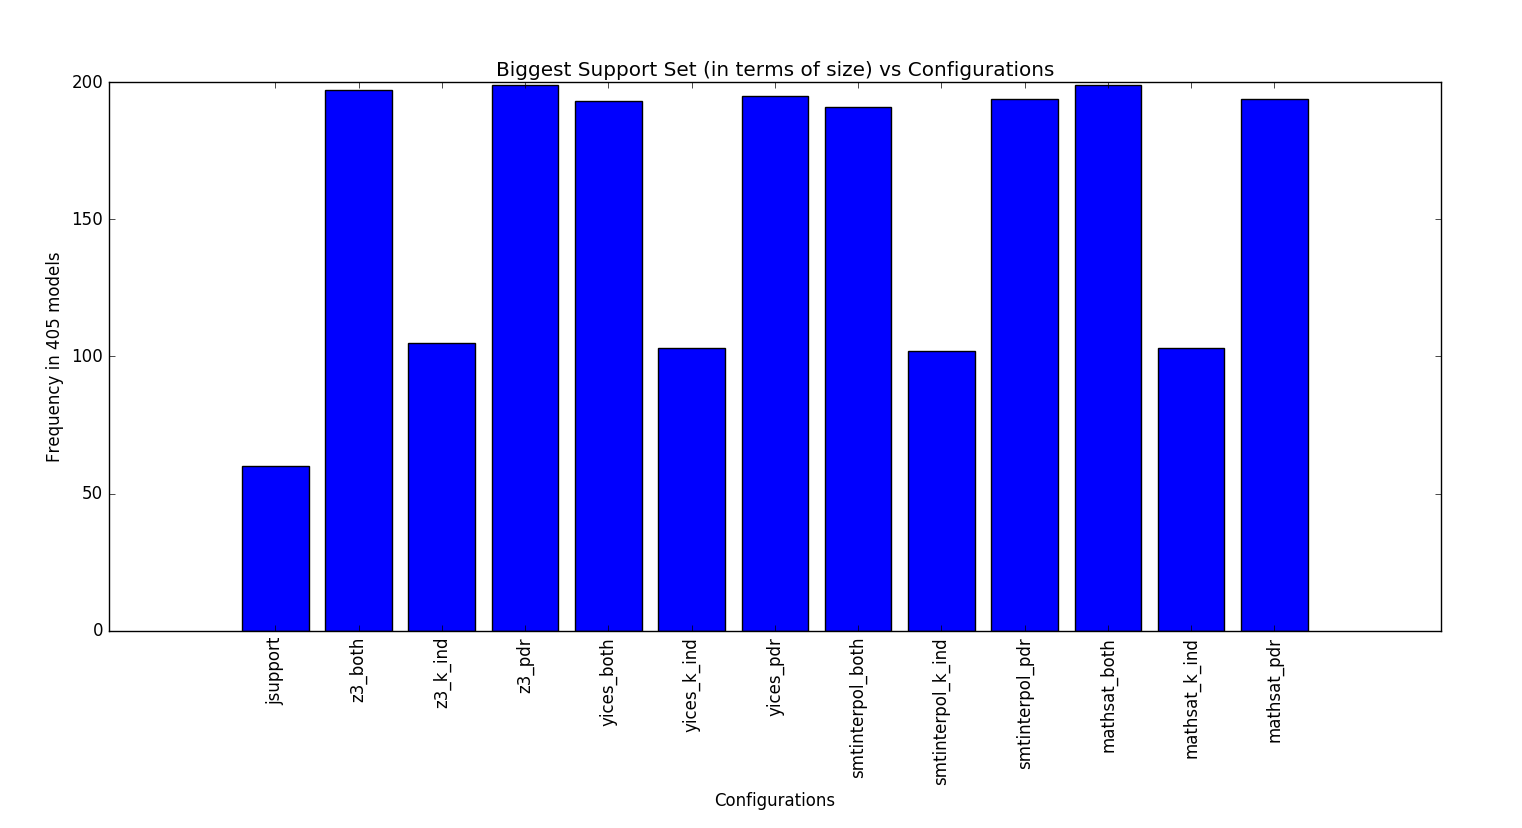
\includegraphics[width=\textwidth]{figs/big_conf.png}
  \caption{\small{Biggest support set (in terms of size) vs configurations}}\label{fig:bigest}
\end{figure}

\vspace{6pt}
\noindent\fbox{%
    \parbox{\textwidth}{%
    Solvers/ proof engines have negligible effects on the size of the support set computed by \texttt{JKind}.
    }%
}
 \vspace{9pt}

\textbf{(2)} Since \texttt{JSupport}, with a great percentage, most of the time computed the smallest support set, we compared the size of the sets computed in each \texttt{JKind} configuration with \texttt{JSupport} per model. Fig~\ref{fig:minpdr} to Fig~\ref{fig:minboth} represent the results. If we take a closer look at the results in the pictures, we can summarize them as shown in Table~\ref{tab:minimality}. For each configuration, we collected the difference between its support size and \texttt{JSupport} per model. Then, minimum, maximum, average, and standard deviation of the collected data have been reported.


\begin{figure}
  \centering
  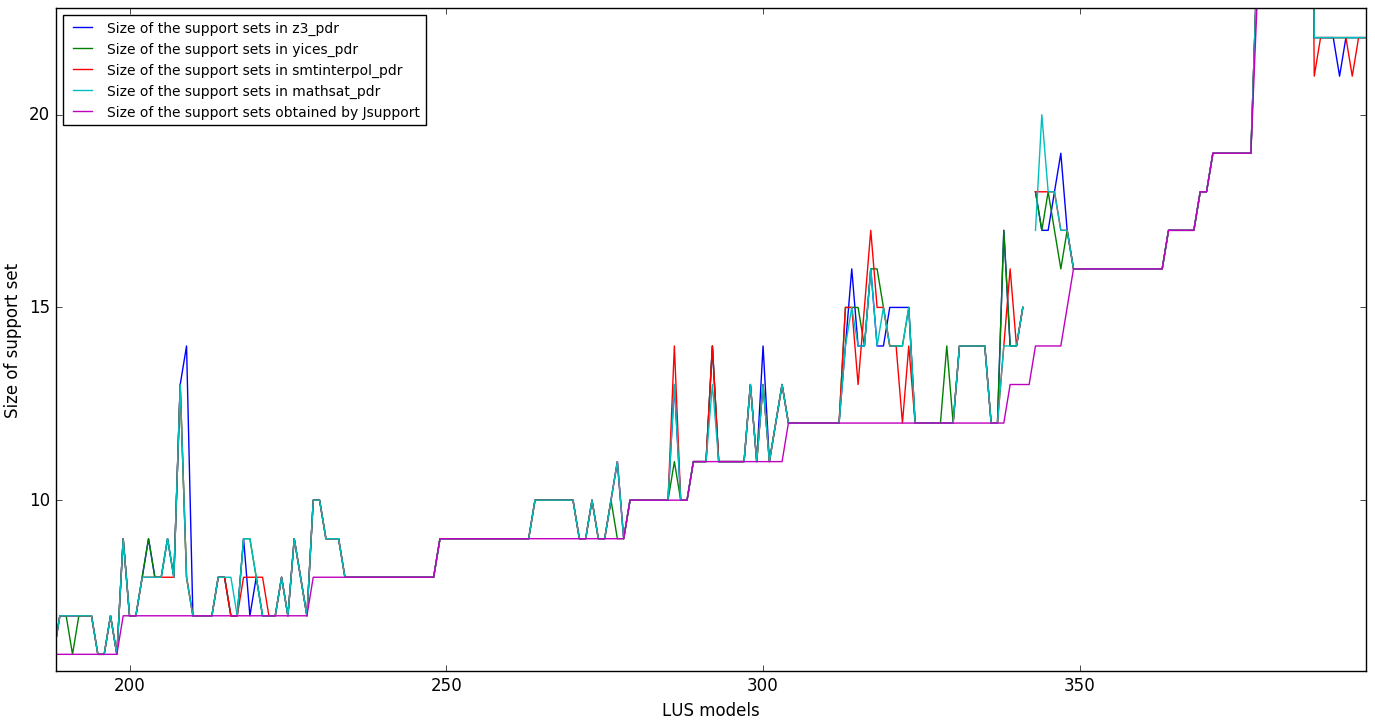
\includegraphics[width=\textwidth]{figs/minimality_pdr.png}
  \caption{\small{Minimality comparison of \texttt{PDR}}}\label{fig:minpdr}
\end{figure}


\begin{figure}
  \centering
  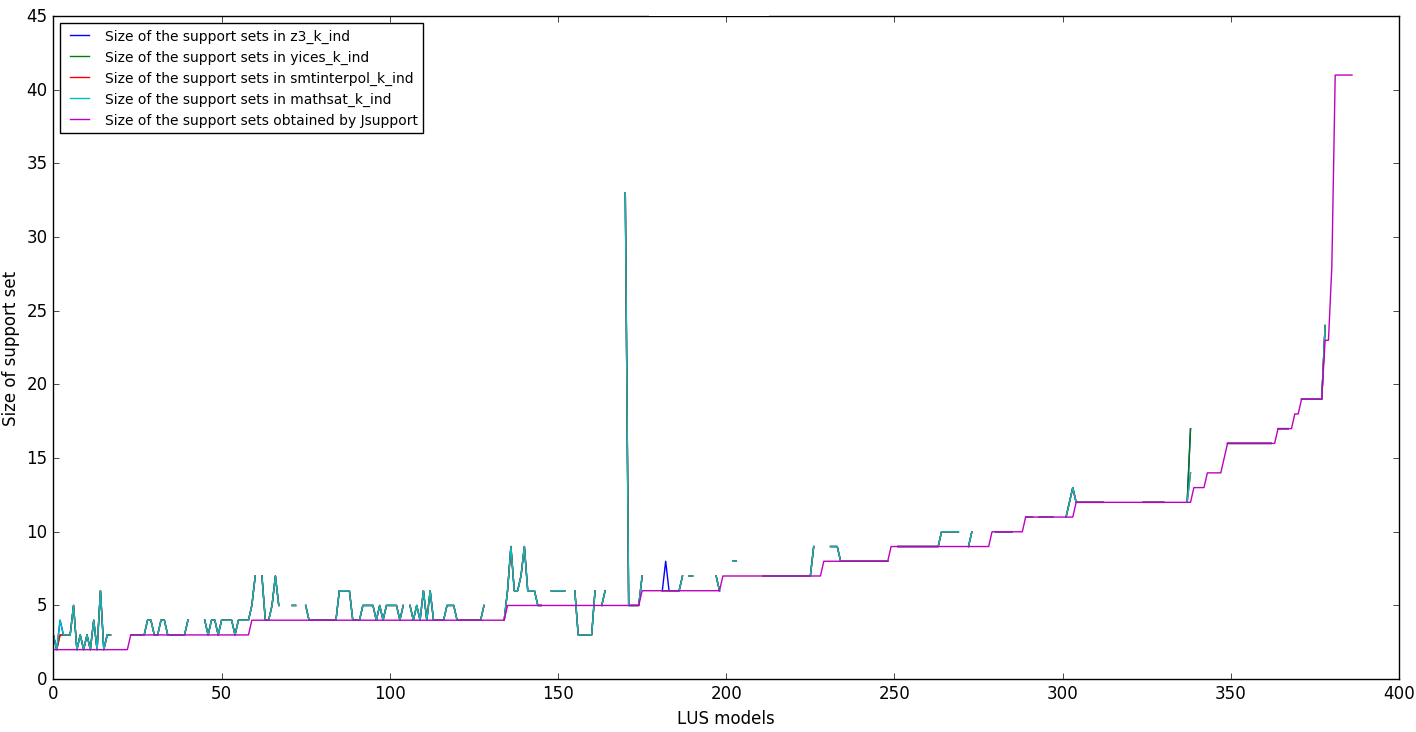
\includegraphics[width=\textwidth]{figs/minimality_kind.png}
  \caption{\small{Minimality comparison of \texttt{K-induction}}}\label{fig:minkind}
\end{figure}


\begin{figure}
  \centering
  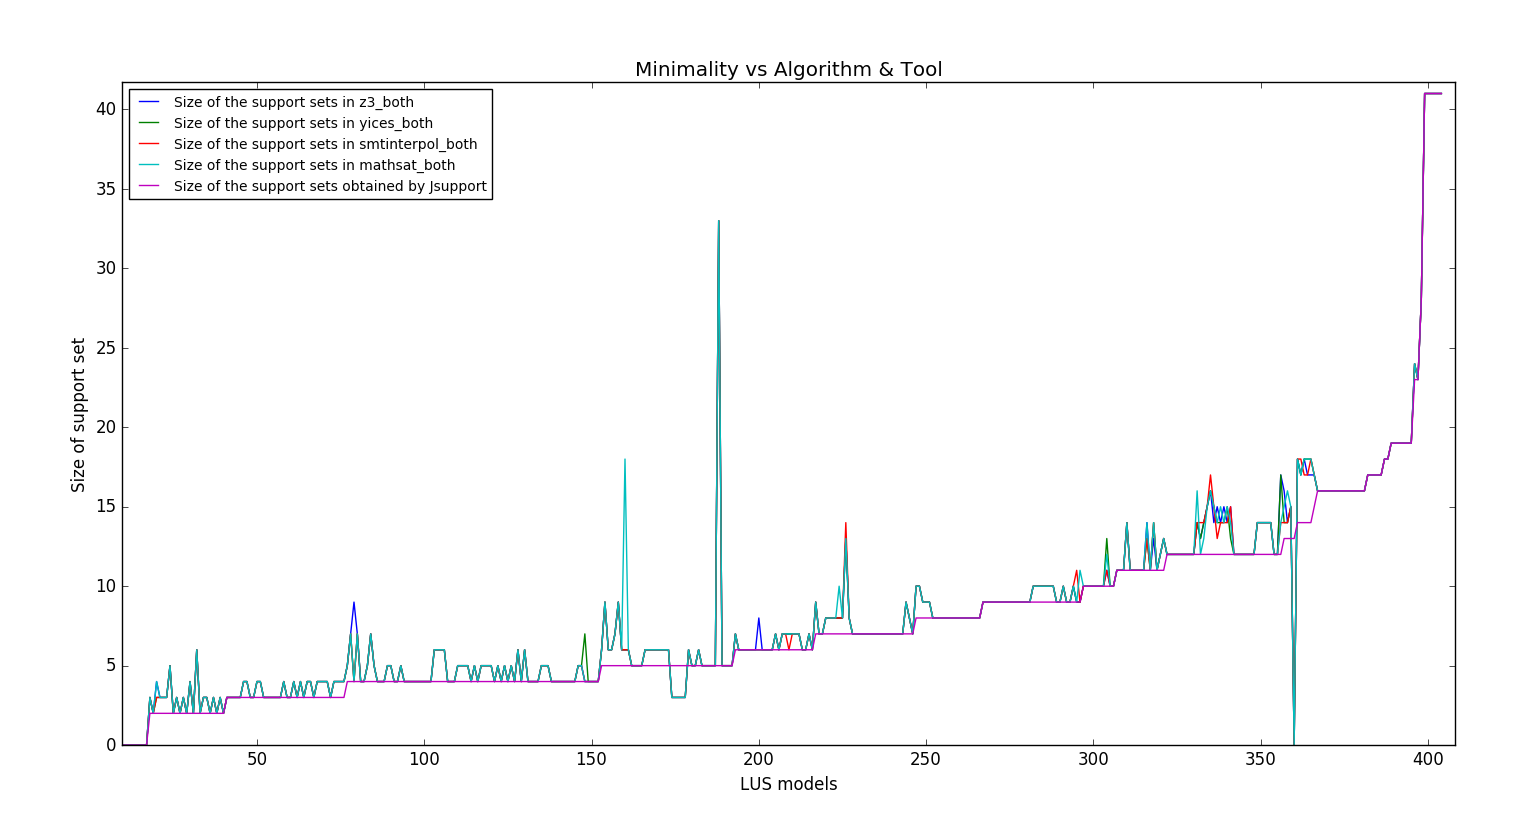
\includegraphics[width=\textwidth]{figs/minimality_both.png}
  \caption{\small{Minimality comparison of \texttt{K-induction} and \texttt{PDR} working together}}\label{fig:minboth}
\end{figure}


\begin{table}
  \centering
  \begin{tabular}{|c|c|c|c|c|}
     \hline
     configuration & min & max & mean & stdev \\[0.5ex]
     \hline\hline
     K-induction & -2 & 28 & 0.542 & 1.831 \\[0.5ex]
     PDR & -2 & 28 & 0.677 & 1.819 \\[0.5ex]
     Both engines & -2 & 28 & 0.661 & 1.751 \\[0.5ex]
     \hline
     Z3, K-ind & -2 & 28 & 0.555 & 1.842 \\[0.5ex]
     Yices, K-ind & -2 & 28 & 0.544 & 1.838 \\[0.5ex]
     SMTInterpol, K-ind & -2 & 28 & 0.534 & 1.822 \\[0.5ex]
     MathSAT, K-ind & -2 & 28 & 0.537 & 1.823 \\[0.5ex]
     \hline
     Z3, PDR & -2 & 28 & 0.697 & 1.852 \\[0.5ex]
     Yices, PDR & -2 & 28 & 0.668 & 1.807 \\[0.5ex]
     SMTInterpol, PDR & -2 & 28 & 0.673 & 1.813 \\[0.5ex]
     MathSAT, PDR & -2 & 28 & 0.668 & 1.803 \\[0.5ex]
     \hline
     Z3, Both engines & -2 & 28 & 0.663 & 1.729 \\[0.5ex]
     Yices, Both engines & -2 & 28 & 0.650 & 1.721 \\[0.5ex]
     SMTInterpol, Both engines & -2 & 28 & 0.637 & 1.713 \\[0.5ex]
     MathSAT, Both engines & -2 & 28 & 0.692 & 1.837 \\[0.5ex]
     \hline     
   \end{tabular}
  \caption{\small{Summary of minimality analyses}}\label{tab:minimality}
\end{table}

\vspace{6pt}
\noindent\fbox{%
    \parbox{\textwidth}{%
     \texttt{JKind} is able to find minimal support sets with a very negligible dependency on solvers/ proof engines.
    }%
}
 \vspace{9pt}

% RQ4: Is there any relationship between the model size and variety of its support sets?
\textbf{RQ4.} The size of the models in our benchmark is between 0 KB and 10 KB. 
We divided the models into 9 different categories based on their sizes such that $category_i$ contains
all models whose sizes are between $(i - 1)$ KB and $i$ KB. Then, using the \textit{similarity} formula defined in RQ2, the similarity for each model in each category was calculated. After that, minimum, maximum, average, standard deviation of the data were obtained per category. Table~\ref{tab:modelsize} summarizes the result of this analysis; the column \emph{number} in the table shows the number of models in each category, which means the sum of the numbers in the column is 405 (for example, there are 6 models whose sizes are between 8 KB and 9 KB, and in all of them \textit{similarity} is 1.0).
 
 
\begin{table}
  \centering
  \begin{tabular}{ |c||c|c|c|c|c|}
    \hline
    size (KB) & number&
     min & max & mean & stdev \\[0.5ex]
    \hline\hline
    [0-1] & 49 & 0.33 & 1.0 & 0.877 & 0.213 \\[0.5ex]
    [1-2] & 90& 0.3 & 1.0 & 0.835 & 0.192 \\[0.5ex]
    [2-3] & 26&0.5 & 1.0 & 0.876 & 0.131 \\[0.5ex]
    [3-4] & 34&0.57 & 1.0 & 0.896 & 0.158 \\[0.5ex]
    [4-5] & 88&0.12 & 1.0 & 0.895 & 0.153 \\[0.5ex]
    [5-6] & 11&0.75 & 1.0 & 0.83 & 0.107 \\[0.5ex]
    [6-7] & 2&0.96 & 1.0 & 0.98 & 0.02 \\[0.5ex]
    [7-8] & 99&0.28 & 1.0 & 0.916 & 0.124 \\[0.5ex]
    [8-9] & 6&1.0 & 1.0 & 1.0 & 0.0 \\[0.5ex]
    \hline
  \end{tabular}
  \caption{Model size vs similarity among its support sets}\label{tab:modelsize}
\end{table}

\vspace{6pt}
\noindent\fbox{%
    \parbox{\textwidth}{%
     The size of the model does not affect the stability of our algorithm; 
     if a model is large, it does not mean that it will have a lot of different minimal support sets. In other words, minimal support sets of a given property computed by \texttt{JKind} will be very similar to each other.
    }%
}
 \vspace{9pt}
 
% RQ5: How close to minimal are the support sets computed by our algorithm? For each model, we have 12 sets of support computed by \texttt{JKind}, and one \emph{minimal} set computed by \texttt{JSupport}; we would like to know which configurations generated sets that are very close or far to the minimal one.

\textbf{RQ5.} To address this question, we analyzed our experimental data from different viewpoints described in the following.

\textbf{(1)} We would like to know which configurations generated sets that are very close or far to the minimal one. To address this question, we calculated pairwise Jaccard distance between sets obtained from different configurations and \texttt{JSupport} per model. Then, minimum, maximum, mean, and standard deviation of the calculated data were obtained among all models. Fig~\ref{fig:jsupjadis} is a summary of this analysis. The result can be also summarized as follows:
\begin{itemize}
  \item minimum of Jaccard distances from \texttt{JSupport} among all models is: 0.0
  \item maximum of Jaccard distances from \texttt{JSupport} among all models is: 0.882
  \item standard deviation for Jaccard distances from \texttt{JSupport} among all models is: 0.034
  \item average of Jaccard distances from \texttt{JSupport} is: 0.103
\end{itemize}


\begin{figure}
  \centering
  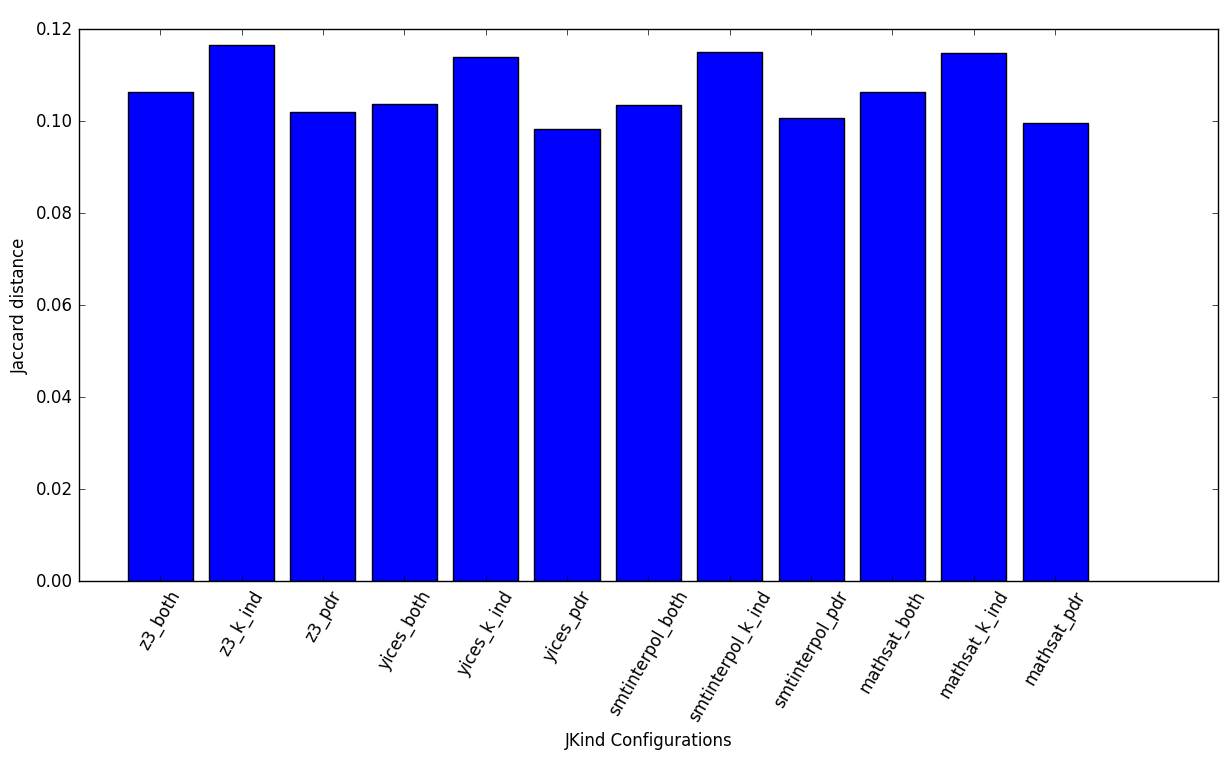
\includegraphics[width=\textwidth]{figs/jsupport_analyses.png}
  \caption{\small{Average Jaccard distance between \texttt{JSupport} and different configurations}}\label{fig:jsupjadis}
\end{figure}

\vspace{6pt}
\noindent\fbox{%
    \parbox{\textwidth}{%
    Using different solvers/ proof engines in \texttt{JKind} has negligible effect on the minimality of the support sets.
    }%
}
 \vspace{9pt}
 
\textbf{(2)} For 405 models, we calculated minimum, maximum, avgerage, and standard deviation of Jaccard distance between JSupport and each configuration
to see which configuration generates support sets close to minimal. 
Table~\ref{tab:jsupconf} represents the result of this analysis; for example, configuration \emph{(Z3, Both)}, shows that \texttt{JKind} with \texttt{Z3} and both \texttt{K-induction} and \texttt{PDR} engines has an average Jaccard distance of 0.106 (in 405 models) from \texttt{JSupport}.


\begin{table}
  \centering
  \begin{tabular}{|c|c|c|c|c|}
    \hline
    configuration & min & max & mean & stdev \\[0.5ex]
    \hline\hline
    Z3, Both & 0.0 & 0.882 & 0.106 & 0.155 \\[0.5ex]
    Z3, K-induction & 0.0 & 0.882 & 0.116 & 0.168 \\[0.5ex]
    z3, PDR & 0.0 & 0.882 & 0.102 & 0.151 \\[0.5ex]
    \hline
    Yices, Both & 0.0 & 0.882 & 0.104 & 0.152 \\[0.5ex]
    Yices, K-induction & 0.0 & 0.882 & 0.114 & 0.166 \\[0.5ex]
    Yices, PDR & 0.0 & 0.882 & 0.098 & 0.147 \\[0.5ex]
    \hline
    SMTInterpol, Both & 0.0 & 0.882 & 0.103 & 0.152 \\[0.5ex]
    SMTInterpol, K-induction & 0.0 & 0.882 & 0.115 & 0.167 \\[0.5ex]
    SMTInterpol, PDR & 0.0 & 0.882 & 0.101 & 0.149 \\[0.5ex]
    \hline
    MathSAT, Both & 0.0 & 0.882 & 0.106 & 0.156 \\[0.5ex]
    MathSAT, K-induction & 0.0 & 0.882 & 0.115 & 0.167 \\[0.5ex]
    MathSAT, PDR & 0.0 & 0.882 & 0.100 & 0.148 \\[0.5ex]
    \hline
  \end{tabular}
  \caption{\small{Jaccard distance between \texttt{JSupport} and each configuration}}\label{tab:jsupconf}
\end{table}

\vspace{6pt}
\noindent\fbox{%
    \parbox{\textwidth}{%
    Different configurations of \texttt{JKind} generated support sets that are very close to minimal sets computed by \texttt{JSupport}.
    }%
}
 \vspace{9pt}

\textbf{(3)} The next approach we took to address this question was to analyze the size of the biggest and smallest support sets versus \texttt{JSupport} per model. The results are shown in Fig~\ref{fig:minjsup}.
We computed the size of the biggest and smallest sets per model, then added them together for all models. The same calculation has been done for JSupport:
\begin{itemize}
  \item the aggregate number of elements in the \emph{smallest} support sets is : 3263
  \item the aggregate number of elements in the \emph{biggest} support sets is: 3609
  \item the aggregate number of elements in support sets computed by \texttt{JSupport} is: 3078
\end{itemize}


\begin{figure}
  \centering
  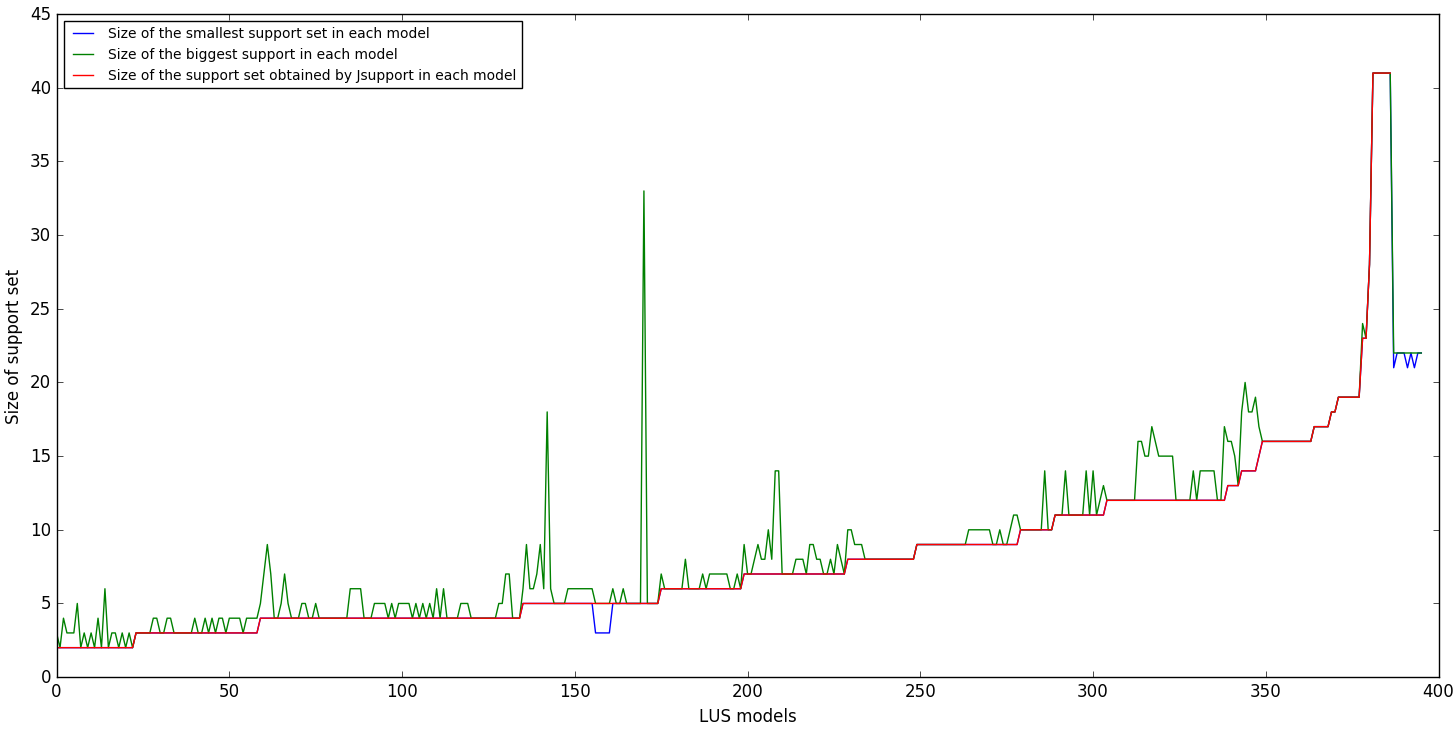
\includegraphics[width=\textwidth]{figs/minimality_analyses.png}
  \caption{\small{Minimality comparison}}\label{fig:minjsup}
\end{figure}

\vspace{6pt}
\noindent\fbox{%
    \parbox{\textwidth}{%
    Average size of sets computed by \texttt{JKind} is 8.55. And, average size of sets computed by \texttt{JSupport} is 7.60. 
    Therefore, in average, support sets computed by \texttt{JKind} are 88\% close to minimal.
    %  (1 - ((8.55 - 7.6)/ 7.6))  * 100 = 87.5%
    }%
}
 \vspace{9pt}
  
 
% RQ6: overall runtime in JSupport and different solvers
\textbf{RQ6.} In addition to overhead, it is also important to know how efficiently \texttt{JKind} performs on computing set of support in comparison with \texttt{JSupport}. Table~\ref{tab:eff-comp-jsup} compares overall runtime of support computation in different solvers and \texttt{JSupport}.


\begin{table}
  \centering
  \begin{tabular}{ |c||c|c|c|c| }
    \hline
     runtime (sec) & min & max & mean & stdev \\[0.5ex]
    \hline\hline
    JSupport & 2.381 & 165.157 & 21.533 & 23.533 \\[0.5ex]
    Z3   & 0.112 & 42.928 & 2.412 & 5.009 \\[0.5ex]
    Yices &   0.111  & 39.657   & 2.464 & 5.224 \\[0.5ex]
    SMTInterpol& 0.225 & 514.886 &  4.331 & 26.411 \\[0.5ex]
    MathSAT & 0.111 & 43.623 &  2.765 & 5.157 \\[0.5ex]
    \hline
  \end{tabular}
  \caption{\small{\texttt{JKind} runtime with \emph{-support} option in different solvers compared with \texttt{JSupport}}}
  \label{tab:eff-comp-jsup}
\end{table}


%For calculations, we considered all settings where both \texttt{K-induction} and \texttt{PDR} were activated
% then in for all 405 models in everything, we collected runtime info, then calculated min/max/avg/stdev between them
% in other words, there were 4 settings to be considered: z3_both, yices_both, mathsat_both, smtinterpol_both
For 405 models, runtime of support computation in the configurations where both \texttt{K-induction} and \texttt{PDR} were activated has been collected. Fig~\ref{fig:runtimez3} and Fig~\ref{fig:runtimeall} visualize the results.


%\begin{figure}
%\centering
%\begin{tabular}[c]{cc}
%    \begin{subfigure}[b]{0.20\textwidth}
%      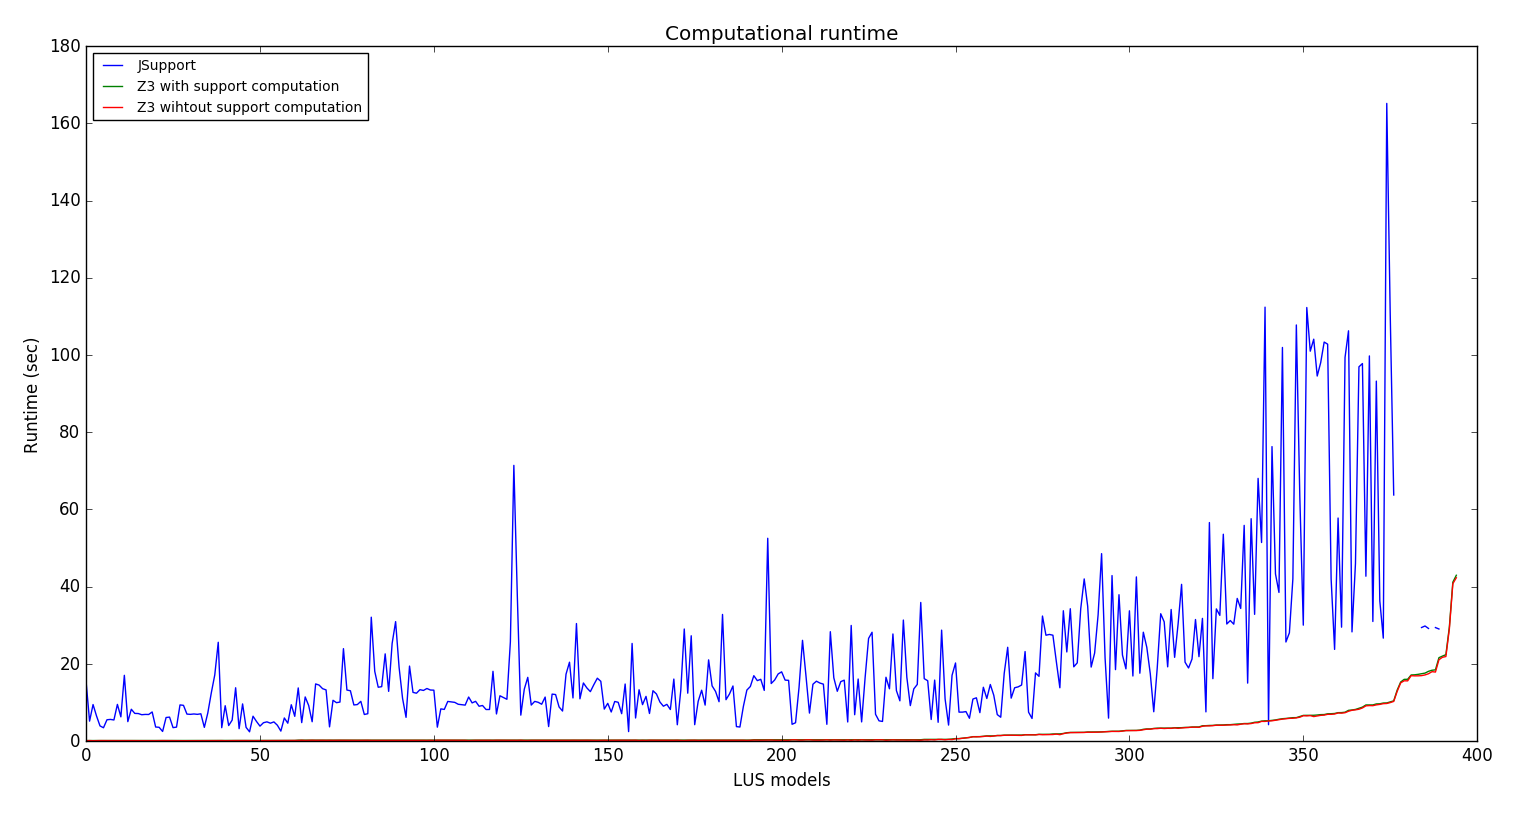
\includegraphics[width=\textwidth]{figs/figure_1.png}
%    \end{subfigure}&
%    \begin{subfigure}[b]{0.20\textwidth}
%      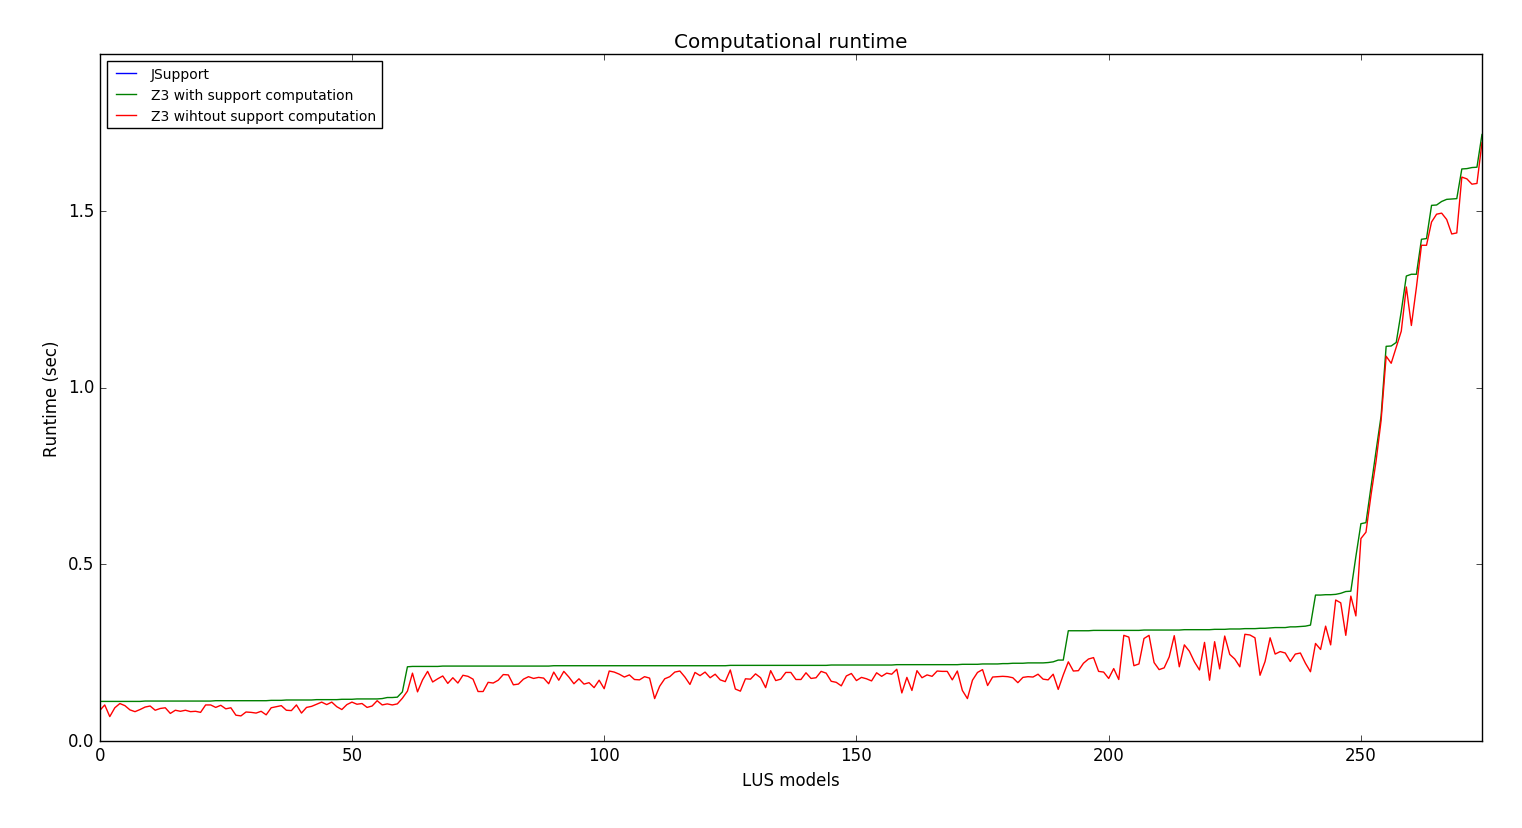
\includegraphics[width=\textwidth]{figs/figure_z3_zoom.png}
%    \end{subfigure}\\
%    \begin{subfigure}[b]{0.20\textwidth}
%      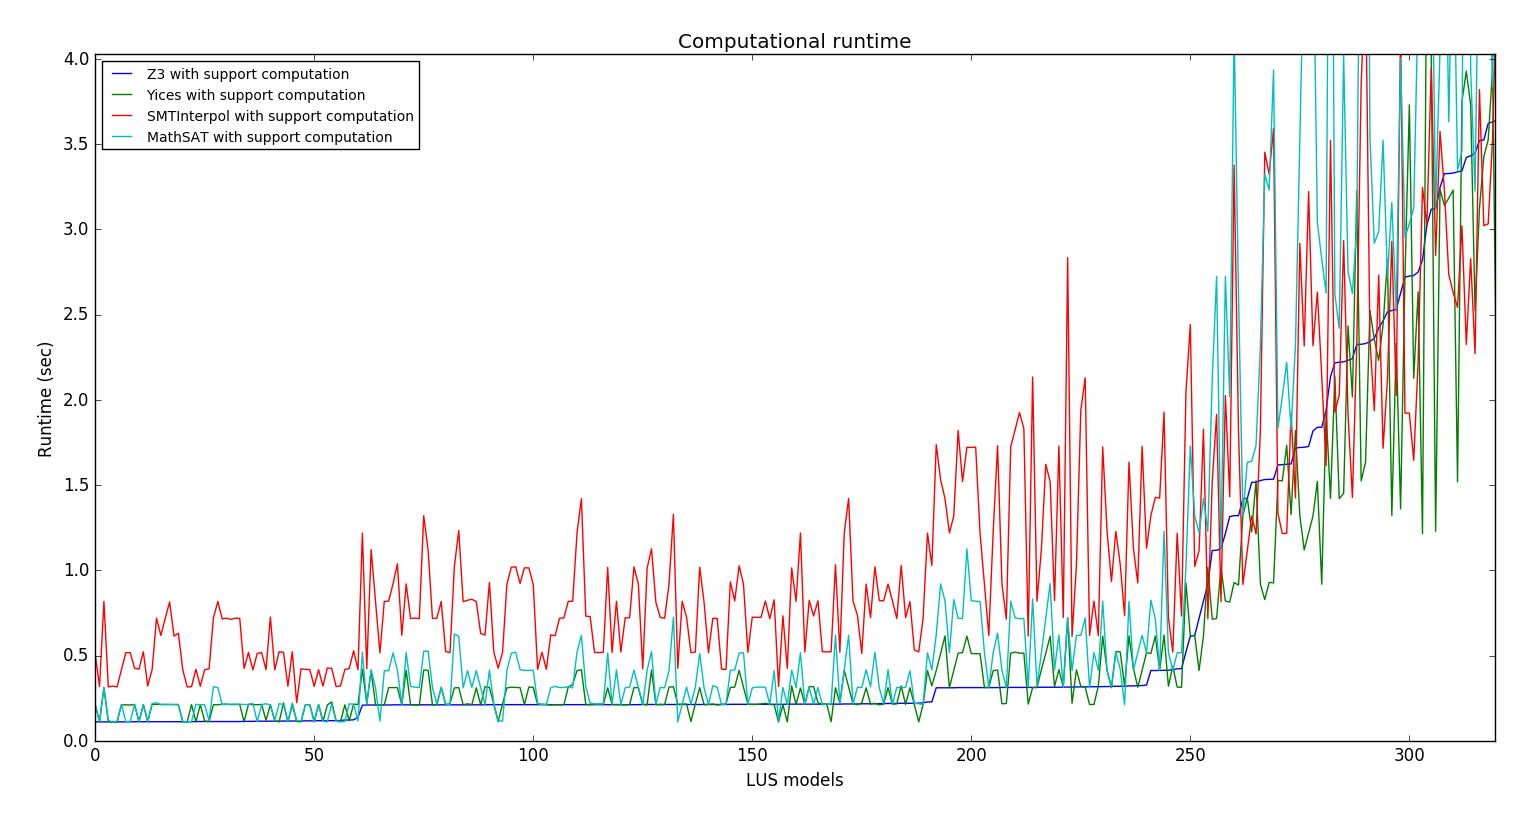
\includegraphics[width=\textwidth]{figs/solvers-support-zoom2.png}
%    \end{subfigure}&
%    \begin{subfigure}[b]{0.20\textwidth}
%      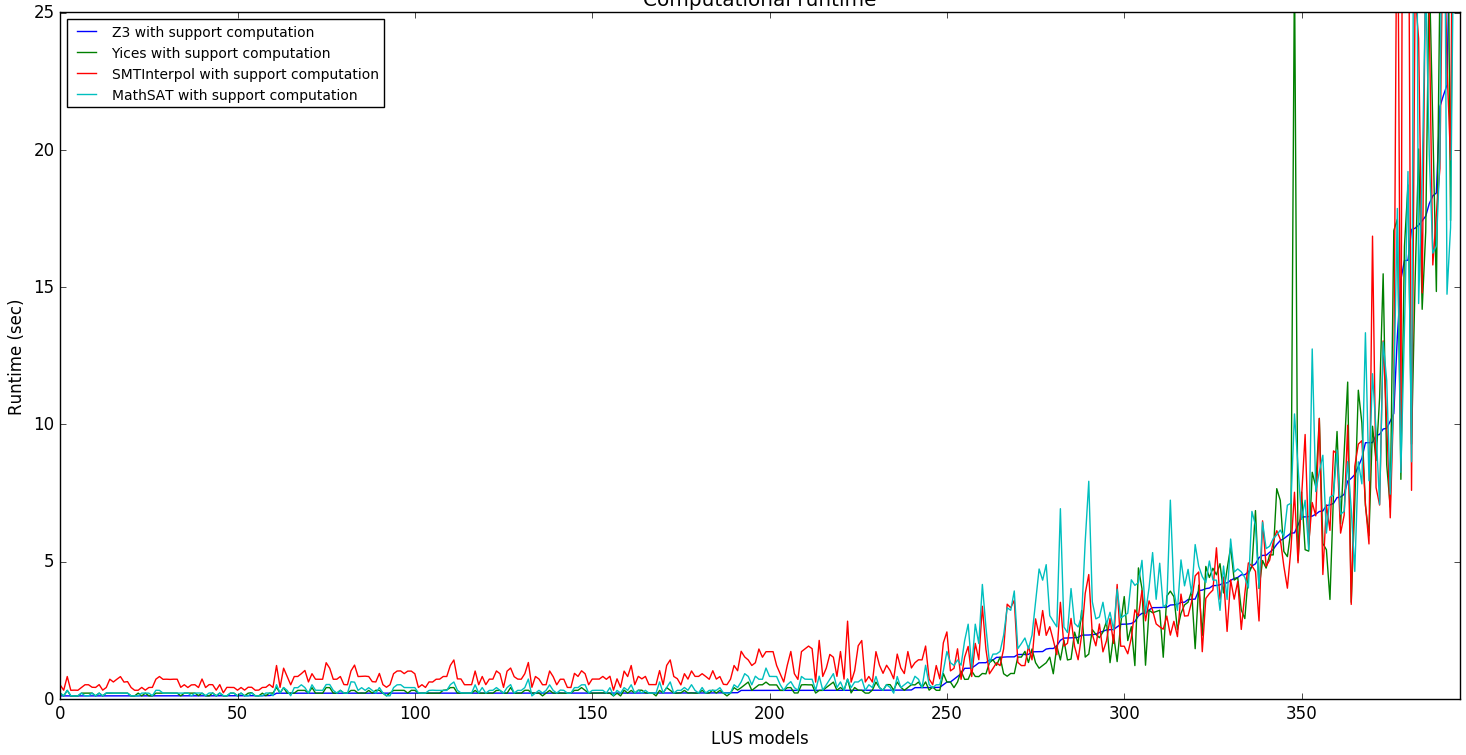
\includegraphics[width=\textwidth]{figs/solvers-support-zoom1.png}
%    \end{subfigure}
%  \end{tabular}
%\caption{\small{Runtime of support computation}}
%\label{fig:runtime}
%\end{figure}
\begin{figure}
  \centering
  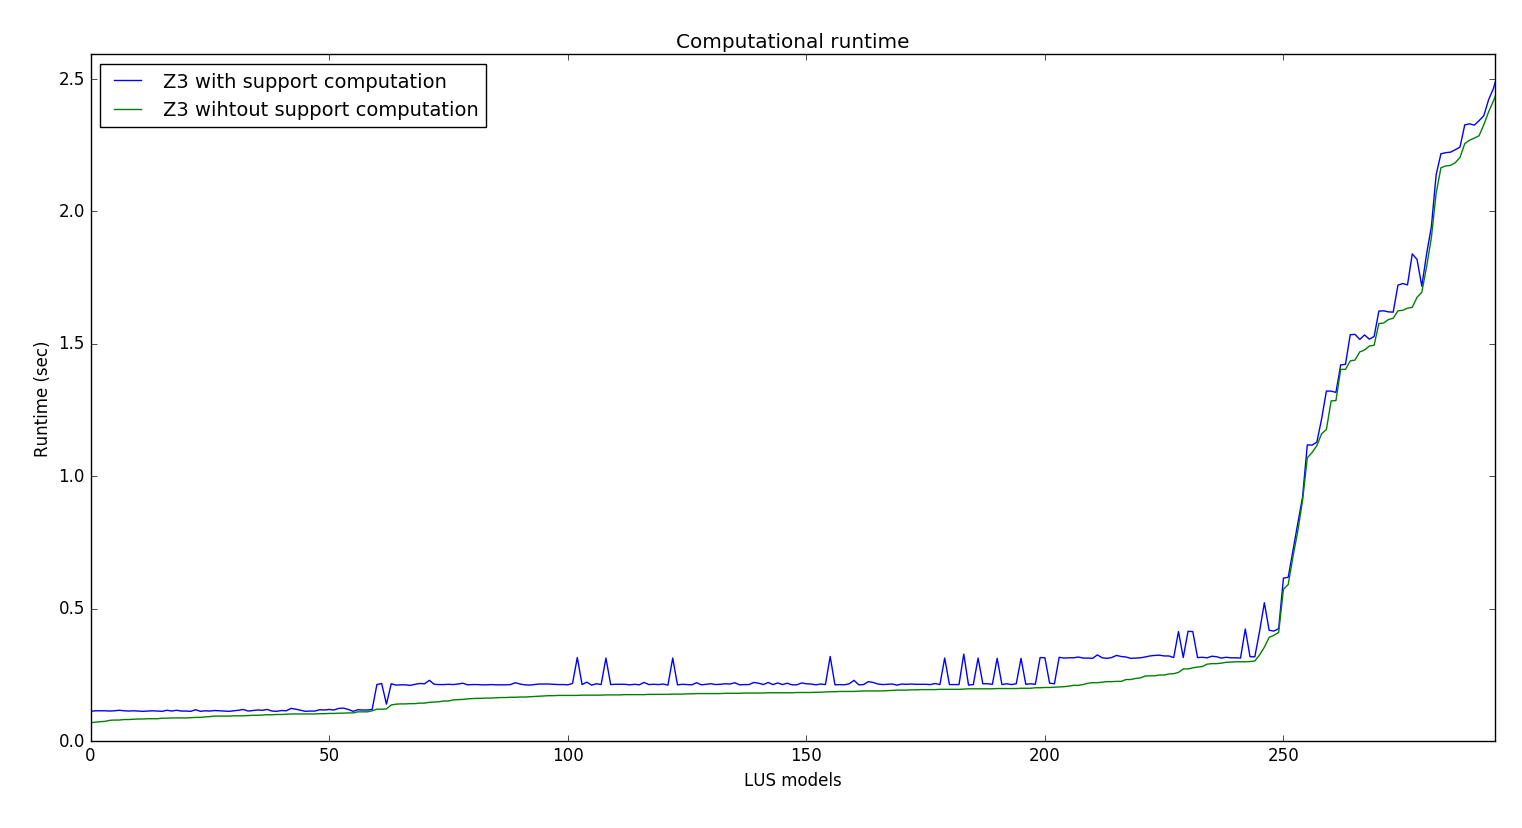
\includegraphics[width=\textwidth]{figs/runtimeZ3.png}
  \caption{\small{Runtime of support computation with \texttt{Z3} and \texttt{JSupport}}}\label{fig:runtimez3}
\end{figure}


\begin{figure}
  \centering
  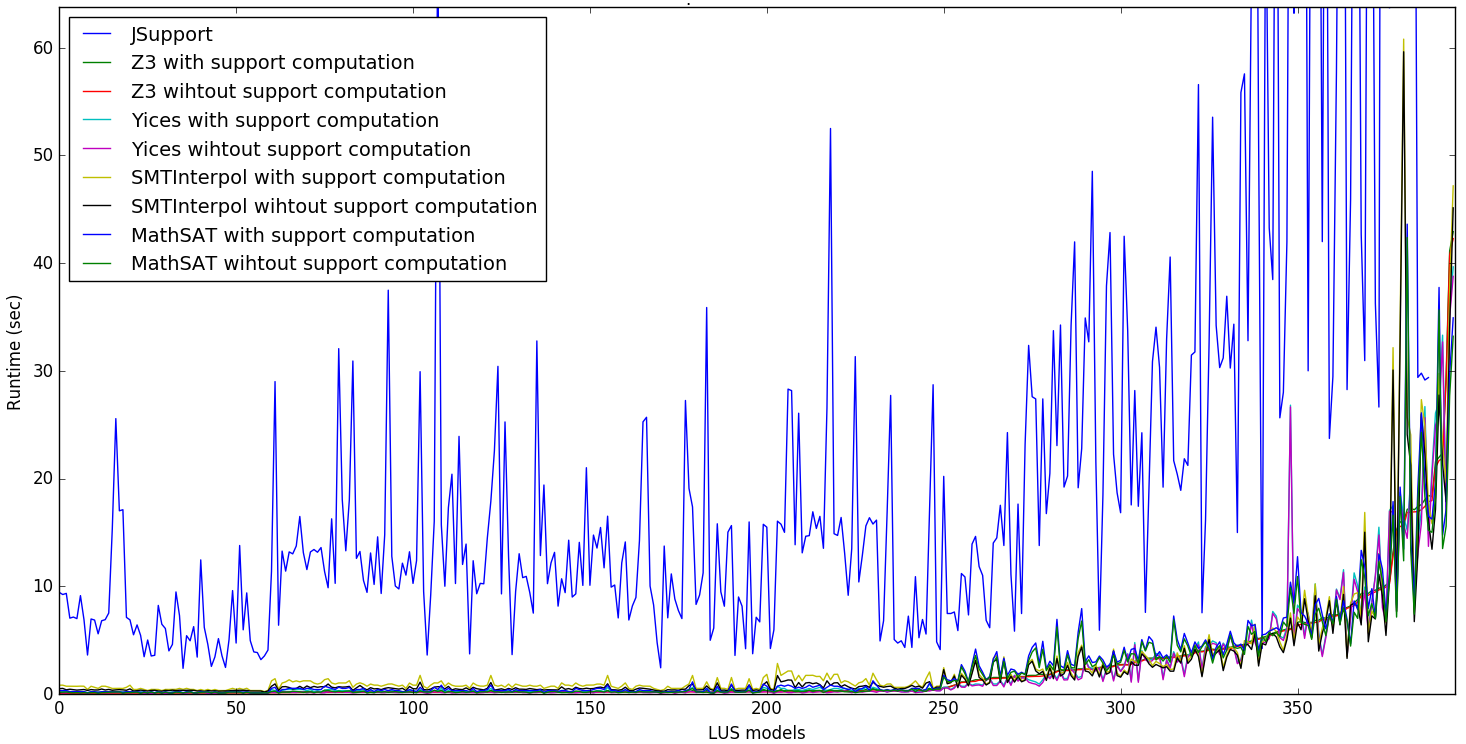
\includegraphics[width=\textwidth]{figs/runtimeAll.png}
  \caption{\small{Runtime of support computation with all solvers}}\label{fig:runtimeall}
\end{figure}


\vspace{6pt}
\noindent\fbox{%
    \parbox{\textwidth}{%
        Time-efficiency of computing support set in \texttt{JKind} is not quite solver-dependent. However, SMTInterpol works less efficiently in comparison with others. 
    }%
}
\noindent\fbox{%
    \parbox{\textwidth}{%
        Support computation by \texttt{JSupport} is much more time-consuming than \texttt{reduce-support} engine.
    }%
}
 \vspace{9pt}
